\chapter{Náhodné veličiny, distribuční a momentová funkce}

\section{Náhodná veličina a kumulativní distribuční funkce}

\begin{definition}[Náhodná veličina]
Pro daný pravděpodobnostní prostor $(\Omega, \mathscr{A}, P[\cdot])$ je náhodná veličina $X$, označovaná také jako $X(\cdot)$, funkcí s definičním oborem hodnot $\Omega$ a reálnou osou jako oborem hodnot. Funkce $X(\cdot)$ musí splňovat podmínku, že množina $A_r = \{\omega: X(\omega) \le r\}$ náleží do $\mathscr{A}$ pro každé reálné číslo $r$.
\end{definition}
Jestliže tuto definici zasadíme do rámce náhodného experimentu, pak
\begin{enumerate}
\item $\Omega$ je úplným souborem všech možných výsledků tohoto experimentu a
\item náhodná veličina $X(\cdot)$ je funkcí s definičním oborem $\Omega$, která přiřazuje reálné číslo každému výsledku náhodného experimentu.
\end{enumerate}
Požadavek, aby $\omega$, pro které platí $X(\omega) \le r$, bylo náhodným jevem (tj. prvkem $\mathscr{A}$), není nikterak omezující, protože naším záměrem je používat pojmu náhodná veličina pouze k popisu náhodných jevů. Jen zřídka kdy se totiž budeme zajímat o náhodnou veličinu jako takovou - předmětem našeho zájmu budou spíše náhodné jevy definované skrze náhodné veličiny.
V následujícím textu budeme pro označení náhodných veličin používat velkých písmen latinské abecedy (např. $X$) a pro označení jejich konkrétních hodnot pak malých písmen latinské abecedy (např. $X = x$).

\begin{example}
Uvažujme hod mincí. Nechť náhodná veličina $X$ označuje počet hlav. Je zřejmé, že $\Omega = \{\textit{orel, hlava}\}$, $X(\omega) = 1$ pro $\omega = \textit{hlava}$ a $X(\omega) = 0$ jestliže $\omega = \textit{orel}$. Náhodná veličina $X$ tak asociuje reálné čéslo s každým možným výsledkem náhodného experimentu. Měli bychom tedy dokázat, že $\{\omega: X(\omega) \le r\}$ náleží do $\mathscr{A}$ pro každé reálné číslo $r$. V našem případě se $\mathscr{A}$ skládá ze čtyř podmnožin - $\emptyset, \textit{\{hlava\}}, \textit{\{orel\}}$ a $\Omega$. Jestliže $r < 0$, pak $\{\omega: X(\omega) \le r\} = \emptyset$. Jestliže $0 \le r < 1$, pak ${\omega: X(\omega) \le r} = \textit{\{orel\}}$. Jestliže $r \ge 1$, pak $\{\omega: X(\omega)\} = \Omega = \textit{\{hlava, orel\}}$. Proto pro každé $r$ náleží množina $\{\omega: X(\omega) \le r\}$ do $\mathscr{A}$ a $X(\cdot)$ je tak náhodnou veličinou.
\end{example}

\begin{definition}[Kumulativní distribuční funkce]
Kumulativní distribuční funkce $F_X(\cdot)$ náhodné veličiny $X$ je definována jako funkce, jejímž definičním oborem je reálná osa a oborem hodnot je interval $[0, 1]$ a která splňuje podmínku $F_X(x) = P[X \le x] = P[X \le x] = P[\{\omega: X(\omega) \le x\}]$ pro každé reálné číslo $x$.
\end{definition}
Každá náhodná veličina je jedinečně definována skrze svou kumulativní distribuční funkci. S pomocí příslušné kumulativní distribuční funkce a s pomocí definice náhodné veličiny lze nalézt pravděpodobnost daného náhodného jevu\footnote{V tomto případě je využito požadavku, aby $\omega: X(\omega) \le r$ náleželo do $\mathscr{A}$.}.

\begin{example}
Uvažujme hod mincí. Nechť náhodná veličina $X$ označuje počet hlav. Kumulativní distribuční funkce je definována jako
\begin{equation*}
F_X(x) =
\begin{cases}
0~~~\textit{pro}~x<0\\
\frac{1}{2}~~~\textit{pro}~x\le x < 1\\
1~~~\textit{pro}~x\ge 1
\end{cases}
\end{equation*}
popř. s využitím idikační funkcí jako
\begin{equation*}
F_X(x) = \frac{1}{2}I_{[0,1)}(x) + I_{[1, \infty)}(x)
\end{equation*}
\end{example}
\begin{definition}[Vlastnosti kumulativní distribuční funkce]
Z výše uvedeného lze vypozorovat, že kumulativní distribuční funkce má následující vlastnosti.
\begin{enumerate}
\item $F_X(-\infty) \equiv \lim_{x \rightarrow -\infty} F_X(x) = 0$ a $F_X(+\infty) \equiv \lim_{x \rightarrow +\infty} F_X(x) = 1$
\item $F_X(\cdot)$ je monotonní, neklesající funkcí. To znamená, že $F_X(a) \le F_X(b)$ pro $a < b$.
\item $F_X(\cdot)$ je spojitá zprava. To znamená, že $\lim_{0 < h \rightarrow 0} F_X(x + h) = F_X(x)$\footnote{Spojitost zprava je dána definicí $F_X(x) = P[X \le x]$. Pokud bychom, jako někteří jiní autoři, použili definici $F_X(x) = P[X < x]$, pak by $F_X(\cdot)$ byla spojitá zleva.}.
\end{enumerate}
\end{definition}

\begin{proof}
Dokažme vlastnost (2). Platí $\{\omega: X(\omega) \le b\} = \{X \le b \} = \{X \le a \} \cup \{ a < X \le b\}$ a $\{X \le a \} \cap \{a < X \le b\} = \emptyset$. Proto $F_X(b) = P[X \le b] = P[X \le a] + P[a < X \le a] = F_X(a)$.
\end{proof}

\begin{definition}[Kumulativní distribuční funkce]
Libovolná funkce $F(\cdot)$ s reálnou osou jako definičním oborem a oborem hodnot $[0, 1]$, která splňuje všechny tři výše uvedené podmínky, je kumulativní distribuční funkce.
\end{definition}

\section{Pravděpodobnostní funkce}

\subsection{Nespojitá náhodná veličina}

\begin{definition} [Nespojitá náhodná veličina]
Náhodná veličina $X$ je nespojitá, jestliže množina hodnot, kterých může nabývat, je spočetná. Jestliže je náhodná veličina $X$ nespojitá, pak je nespojitá také její kumalativní distribuční funkce $F_X(\cdot)$. Vedle pojmu nespojitá náhodná veličina se někdy používá také pojem diskrétní náhodná veličina.
\end{definition}

Spočetnou množinou rozumíme množinu, která má konečný popř. spočetný počet prvků $x_1, x_2, ...$. Jestliže náhodná veličina $X$ nabývá náhodných hodnot z takovéto množiny, pak $\Omega = \bigcup_n \{\omega: X(\omega) = x_n\} = \bigcup_n \{X = x_n \}$ a $\{X = x_i\} \cap \{X = x_j\} = \emptyset$ pro $i \not= j$. Proto na základě třetího aximu pravděpodobnosti platí $1 = P[\Omega] = \sum_n P[X = x_n]$.

\begin{definition}[Pravděpodobnostní funkce nespojité náhodné veličiny]
Uvažujme náhodnou veličinu $X$, která může nabývat hodnot $x_1, x_2, ..., x_n, ...$. Pak funkce $f_X(\cdot)$ definovaná jako
\begin{equation*}
f_X(x) =
\begin{cases}
P[X = x_j]~~~\textit{pro}~x=x_j, j = 1, 2, ..., n, ...\\
0~~~\textit{pro}~x \not= x_j
\end{cases}
\end{equation*}
je nespojitou pravděpodobnostní funkcí nespojité náhodné veličiny $X$.
\end{definition}

Hodnoty $x_1, x_2, ...$, kterých může nespojitá náhodná veličina $X$ nabývat, nazýváme body koncentrace. Hodnotu pravděpodobnostní funce $f_X(x_j)$ pak nazýváme koncentrací v bodě $x_j$.

\begin{theorem}
Nechť je $X$ nespojitou náhodnou veličinou. Platí, že $F_X(\cdot)$ lze získat z $f_x(\cdot)$ a naopak.
\end{theorem}

\begin{proof}
Označme hodnoty náhodné veličiny $X$ jako $x_1, x_2, ...$.
\begin{enumerate}
\item  Jestliže je dáno $f_X(\cdot)$, pak $F_X(x) = \sum_{j:x_j \le x} f_X(x_j)$.
\item Jestliže je dáno $F_X(x)$, pak $f_X(x_j) = F_X(x_j) - \lim_{h \rightarrow 0^+} F_X(x_j - h)$. $f_X(x_j)$ lze tímto způsobem nalézt pro všechny body koncentrace $x_j$ a $f_X(x) = 0$ pro $x \not= x_j, j = 1, 2, ...$, čímž jsme definovali $f_X(x)$ pro všechna reálná čísla.
\end{enumerate}
\end{proof}

\begin{example}
Uvažujme hod hrací kostkou. Náhodná veličina $X$, která představuje hodnotu hodu, má množinu bodů koncentrace $\{1, 2, 3, 4, 5, 6\}$. Odpovídající nespojitá pravděpodobnostní funkce a kumulativní distribuční funkce jsou pak definovány jako
\begin{equation*}
f_X(x_j) = \frac{1}{6}~~~\textit{pro}~j = 1, 2, ..., 6
\end{equation*}
\begin{equation*}
F_X(x_j) = \frac{j}{6}~~~\textit{pro}~j = 1, 2, ..., 6
\end{equation*}
\end{example}

\figure[h]\centering
\begin{pspicture}(11.0,5.0)
    \psline[arrows=->](0.5,0.5)(5.0,0.5)
    \psline[arrows=->](0.5,0.5)(0.5,4.5)
    \rput(0.0,4.8){\psframebox*{$f_X(x)$}}
    \rput(5.0,0.2){\psframebox*{$x$}}

    \psline[arrows=-*](1.1,0.4)(1.1,1.2)
    \psline[arrows=-*](1.7,0.4)(1.7,1.2)
    \psline[arrows=-*](2.3,0.4)(2.3,1.2)
    \psline[arrows=-*](2.9,0.4)(2.9,1.2)
    \psline[arrows=-*](3.5,0.4)(3.5,1.2)
    \psline[arrows=-*](4.1,0.4)(4.1,1.2)
    \rput(1.1,0.2){\psframebox*{\tiny{1}}}
    \rput(1.7,0.2){\psframebox*{\tiny{2}}}
    \rput(2.3,0.2){\psframebox*{\tiny{3}}}
    \rput(2.9,0.2){\psframebox*{\tiny{4}}}
    \rput(3.5,0.2){\psframebox*{\tiny{5}}}
    \rput(4.1,0.2){\psframebox*{\tiny{6}}}

    \psline[arrows=->](5.5,0.5)(10.5,0.5)
    \psline[arrows=->](5.5,0.5)(5.5,4.5)
    \rput(5.0,4.8){\psframebox*{$F_X(x)$}}
    \rput(10.5,0.2){\psframebox*{$x$}}

    \psline[arrows=*-o](6.1,1.2)(6.8,1.2)
    \psline[arrows=*-o](6.8,1.9)(7.5,1.9)
    \psline[arrows=*-o](7.5,2.6)(8.2,2.6)
    \psline[arrows=*-o](8.2,3.3)(8.9,3.3)
    \psline[arrows=*-o](8.9,3.9)(9.6,3.9)
    \psline[arrows=*-o](9.6,4.5)(10.3,4.5)
    \psline(6.1,0.4)(6.1,0.6)
    \psline(6.8,0.4)(6.8,0.6)
    \psline(7.5,0.4)(7.5,0.6)
    \psline(8.2,0.4)(8.2,0.6)
    \psline(8.9,0.4)(8.9,0.6)
    \psline(9.6,0.4)(9.6,0.6)
    \rput(6.1,0.2){\psframebox*{\tiny{1}}}
    \rput(6.8,0.2){\psframebox*{\tiny{2}}}
    \rput(7.5,0.2){\psframebox*{\tiny{3}}}
    \rput(8.1,0.2){\psframebox*{\tiny{4}}}
    \rput(8.9,0.2){\psframebox*{\tiny{5}}}
    \rput(9.6,0.2){\psframebox*{\tiny{6}}}

  \end{pspicture}
  \label{prob_cum_function}
  \caption{Hod hrací kostkou: Pravděpodobnostní funkce a kumulativní distribuční funkce}
\endfigure

Z obrázku (\ref{prob_cum_function}) je patrné, že kumulativní distribuční funkce nespojité náhodné veličiny $X$ je skoková v bodech koncentrace, tj. že v bodě $x_j$ skokově změní hodnotu o $f_X(x_j)$. Mezi jednotlivými body koncentrace je pak $F_X(\cdot)$ konstantní.

\begin{definition}[Nespojitá pravděpodobnostní funkce]
Libovolná funkce $f(\cdot)$ s reálnou osou jako definičním oborem a oborem hodnot $[0, 1]$ je nespojitou (popř. diskrétní) pravděpodobnostní funkcí, jestliže pro určitou spočetnou množinu $x_1, x_2, ...$ platí
\begin{enumerate}
\item $f(x_j) > 0$ pro $j = 1, 2, ...$
\item $f(x) = 0$ pro $x \not= x_j, j = 1, 2, ...$
\item $\sum f(x_j) = 1$ kde suma je přes body $x_1, x_2, ...$
\end{enumerate}
\end{definition}


\subsection{Spojitá náhodná veličina}

\begin{definition}[Spojitá náhodná veličina]
Náhodnou veličinu $X$ nazýváme spojitou, jestliže existuje funkce $f_X(\cdot)$ taková, že $F_X(x) = \int_{-\infty}^x f_X(u)du$ pro každé reálné číslo $x$. 
\end{definition}

\begin{definition}[Pravděpodobnostní funkce spojité náhodné veličiny]
Jestliže je $X$ spojitá náhodná veličina, pak je funkce $f_X(\cdot)$ ze vztahu $F_X(x) = \int_{-\infty}^xf_X(u)du$ nazývána pravděpodobnostní funkcí náhodné veličiny $X$.
\end{definition}

Pokud bychom slepě lpěli na definici, pak pravděpodobnostní funkce $f_X(\cdot)$ spojité náhodné veličiny $X$ není jedinečná. Např. kumulativní distribuční funkce $F_X(x) = xI_{[0,1)}(u)+I_{[1, \infty)}(x)$ je ``kompatibilní'' s pravděpodobnostní funkcí $f_X(u) = I_{(0,1)}(u)$ i s pravděpodobnostní funkcí $f_X(u) = I_{(0, \frac{1}{2})}(u)+69I_{\frac{1}{2}}(u) + I_{(\frac{1}{2}, 1)}(u)$. V praxi je však jedinečnost pravděpodobnostní funkce daná požadavky na její spojitost.

\begin{theorem}
Nechť je $X$ spojitou náhodnou veličinou. Pak $F_X(\cdot)$ lze odvodit z $f_X()$ a naopak.
\end{theorem}

\begin{proof}
Jestliže $X$ je spojitá náhodná veličina a $f_X(\cdot)$ je dána, pak lze $F_X(x)$ odvodit integrací $f_X(\cdot)$, tj. $F_X(x) = \int_{-\infty}^x f_X(u)du$. Pokud je dáno $F_X(\cdot)$, pak lze $f_X(x)$ odvodit derivací, tj. $f_X(x) = dF_X(x)/dx$ pro ty body $x$, ve kterých pro $F_X(x)$ existuje derivace.
\end{proof}

Značení pro spojitou a nespojitou pravděpodobnostní funkci jsou shodná, přesto mají odlišnou interpretaci. Pro nespojitou náhodnou veličinu je $f(x)$ definováno jako
\begin{equation*}
f_X(x) = P[X = x]
\end{equation*}
Pro spojitou veličinu platí
\begin{equation*}
f_X(x) = \frac{d F_X(x)}{dx} = \lim_{\Delta x \rightarrow 0} \frac{F_X(x + \Delta x) - F_X(x - \Delta x)}{2 \Delta x}
\end{equation*}
a proto $f_X(x)2 \Delta x \approx F_X(x + \Delta x) - F_X(x - \Delta x) = P[x - \Delta x < X \le x + \Delta x]$, což znamená, že pravděpodobnost, že se $X$ nachází v malém intervalu obsahujícím hodnotu $x$, je rovna $f_X(x)$ krát délka tohoto intervalu. Pro nespojitou náhodnou veličinu je $f_X(\cdot)$ funkcí s reálnou osou jako definičním oborem a intervalem $[0, 1]$ jako oborem hodnot. V případě spojité náhodné veličiny je $f_X(\cdot)$ funkcí s reálnou osou jako definičním oborem a intervalem $[0, \infty)$ jako oborem hodnot.

\begin{example}
Nechť náhodná veličina $X$ představuje délku telefonního hovoru. Předpokládejme, kumulativní distribuční funkce $X$ je $F_X(x) = (1 - e^{-\lambda x})I_{[0, \infty)}(x)$, kde $\lambda > 0$. Odpovídající pravděpodobnostní funkce je $f_X(x) = \lambda e^{-\lambda x}I_{[0, \infty)}(x)$. Jestliže je délka hovoru měřena v minutách, pak pro $\lambda = \frac{1}{5}$ je $P[5 < X \le 10] = \int_5^{10} \lambda e^{-\lambda x}dx = e^{-5 \lambda} - e^{-10 \lambda} = e^{-1} - e^{-2} \approx 0.23$. Analogicky lze tuto pravděpodobnost vyjádřit jako $P[5 < X \le 10] = P[X \le 10] - P[X \le 5] = (1 - e^{-10 \lambda}) - (1 - e^{-5 \lambda}) = e^{-1}- e^{-2}$.
\end{example}

Pravděpodobnostní funkci je možné použít pro výpočet pravděpodobnosti jevů definovaných pomocí spojité náhodné veličiny $X$. Např. $P[a < X \le b] = \int_a^b f_X(x)dx$ pro $a < b$.

\begin{definition}[Spojitá pravděpodobnostní funkce]
Libovolná funkce $f(\cdot)$ s reálnou osou jako definičním oborem a $[0, \infty)$ jako oborem hodnot je spojitou pravděpodobnostní funkci tehdy a jen tehdy, jestliže
\begin{enumerate}
\item $f(x) \ge 0$ pro všechna $x$
\item $\int_{-\infty}^{\infty}f(x)dx = 1$
\end{enumerate}
\end{definition}

\subsection{Ostatní náhodné veličiny}

Ne všechny náhodné veličiny jsou buďto spojité nebo nespojité a ne všechny kumulativní distribuční funkce jsou buďto absolutně spojité nebo nespojité. V praxi existuje řada případů, kdy je kumulativní distribuční funkce částečně spojitá a částečně nespojitá. Příkladem může být čekání na semaforu - pokud svítí zelená, je doba čekání rovna nule; pokud svítí červená, záleží doba čekání na tom, ve které fázi jsme na křižovatku dorazili. Situaci ilustruje obrázek (\ref{cross-road}).

\begin{figure}[htp]
\centering
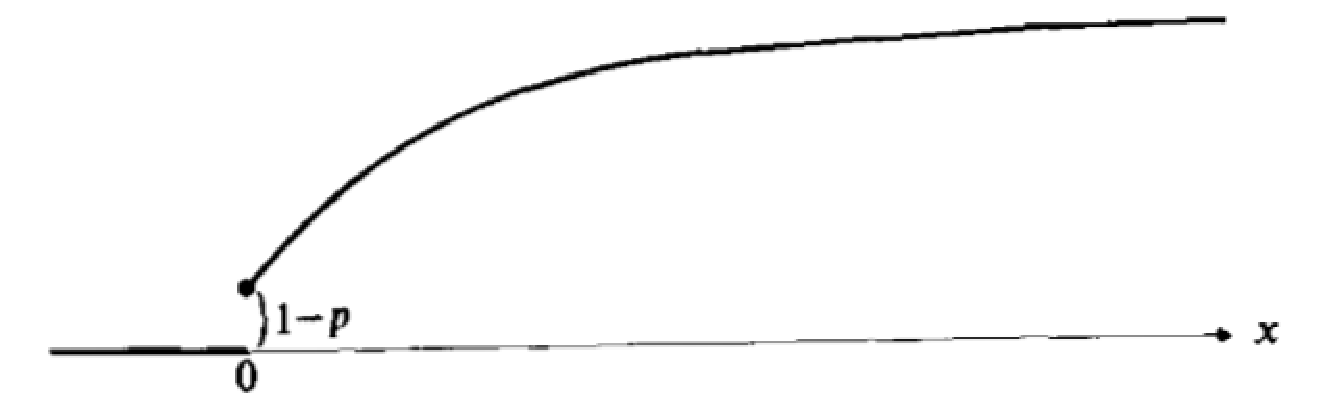
\includegraphics[scale = 0.5]{pictures/partially_continuous_and_discrete.eps}
\caption{Kumulativní distribuční funkce se skokem v $x = 0$ a spojitá pro $x > 0$}
\label{cross-road}
\end{figure}

Vedle toho existuje tzv. singulárně spojitá kumumlativní distribuční funkce, jejichž derivace je téměř ve všech bodech rovna nule. Tento typ kumulativní distribuční funkce je použit v následujícím tvrzení.
\begin{corollary}
Jakákoliv kumulativní distribuční funkce $F(x)$ může být vyjádřena ve formě
\begin{equation*}
F(x) = p_1 F^d(x) + p_2 F^{ac}(x) + p_3 F^{sc}(x)
\end{equation*}
kde $p_i \ge 0,~i = 1, 2, 3$, $\sum_{i=1}^3p_i = 1$, $F^d(\cdot)$ je nespojitá, $F^{ac}(\cdot)$ je absolutně spojitá a $F^{sc}(\cdot)$ je singulárně spojitá kumulativní distribuční funkce.
\end{corollary}

\begin{example}
Uvažujme $F_X(x) = (1-pe^{-\lambda x})I_{[0, \infty)}(x)$. Tuto kumulativní distribuční funkci lze rozepsat do tvaru
\begin{gather*}
F_X(x) = (1-p)F^d(x) + pF^{ac}(x) = (1-p)I_{[0,\infty)}(x) + p(1-e^{-\lambda x})I_{[0,\infty)}(x)\\
= (1 - pe^{-\lambda x})I_{[0, \infty]}(x)
\end{gather*}
\end{example}

Uvažujme $F(x) = (1-p)F^d(x) + pF^{ac}(x)$, kde $0 < p < 1$, $F^d(\cdot)$ je nespojitá a $F^{ac}(\cdot)$ je absolutně spojitá kumulativní distribuční funkce. Odpovídající pravděpodobnostní funkce je definováná jako $f(x) = (1-p)f^d(x) + p f^{ac}(x)$, kde $f^d(\cdot)$ je nespojitá pravděpodobnostní funkce odpovídající funkci $F^{d}(\cdot)$ a $f^{ac}(\cdot)$ je absolutně spojitá pravděpodobnostní funkce odpovídající funkci $F^{ac}(\cdot)$. Tato částečně nespojitá a částečně absolutně spojitá pravděpodobnostní funkce může být poměrně komplikovaná na interpretaci, a proto v takovýchto případech budeme spíše pracovat s kumulativní distribuční funkcí.

\section{Střední hodnoty a momenty}

\subsection{Střední hodnota}

\begin{definition}[Střední hodnota]
Uvažujme náhodnou veličinu $X$. Střední hodnota $X$, označovaná jako $E[X]$ popř. jako $\mu_x$, je definována následujím způsobem.
\begin{enumerate}
\item Jestliže je $X$ nespojité, pak
\begin{equation*}
E[X] = \sum x_j f_X(x_j)
\end{equation*}
pro body koncentrace $x_1, x_2, ..., x_j, ...$.
\item Jestliže je $X$ spojité, pak
\begin{equation*}
E[X] = \int_0^{\infty}x f_X(x)dx
\end{equation*}
\item Pro libovolné $X$ pak platí
\begin{equation*}
E[X] = \int_0^{\infty}[1 - F_X(x)]dx - \int_{-\infty}^0 F_X(x)dx
\end{equation*}
\end{enumerate}
V případě (1) $E[X]$ existuje, jestliže je daná řada absolutně konvergentní. V případě (2) $E[X]$ existuje, jestliže daný integrál existuje. Konečně, v případě (3) existuje $E[X]$, pokud jsou oba integrály konečné.
\end{definition}

Z definicí (1) a (2) je patrné, že na $E[X]$ je možné pohlížet jako na vážený průměr jednotlivých hodnot, kterých může náhodná veličina $X$ nabývat, přičemž vahami jsou příslušné pravděpodobnostni reprezentované pravděpodobnostní funkcí $f_X(x)$ popř. $f_X(x)dx$.

\begin{example}
Uvažujme hod hrací kostkou. Střední hodnota náhodné veličiny $X$, která představuje hodnotu hodu, je rovna
\begin{equation*}
E[X] = \sum_{i = 1}^6 i \frac{1}{6} = \frac{7}{2}
\end{equation*}
\end{example}

\begin{example}
Nechť je $X$ náhodná veličina s pravděpodobnostní funkcí $f_X(x) = \frac{1}{x^2}I_{[1,\infty)}(x)$. Pak
\begin{equation*}
E[X] = \int_1^{\infty} x \frac{1}{x^2}dx=\lim_{b \rightarrow \infty} \ln b = \infty
\end{equation*}
a proto $E[X]$ neexistuje.
\end{example}

\begin{example}
Nechť je $X$ náhodná veličina s kumulativní distribuční funkcí $F_X(x) = (1 - pe^{-\lambda x})I_{[0, \infty)}(x)$. Pak
\begin{equation*}
E[X] = \int_0^{\infty} [1 - F_X(x)]dx - \int_{-\infty}^0F_X(x)dx = \int_0^{\infty} p e^{-\lambda x}dx = \frac{p}{\lambda}
\end{equation*}
\end{example}

\subsection{Rozptyl}

\begin{definition}[Rozptyl]
Nechť je $X$ náhodná veličina se střední hodnotou $E[X]$. Roztyl této náhodné veličiny označovaný jako $D[X]$ resp. jako $\sigma_X^2$, je definován následujícím způsobem.
\begin{enumerate}
\item Jestliže je $X$ nespojité s body koncentrace $x_1, x_2, ..., x_n, ...$, pak
\begin{equation*}
D[X] = \sum_i(x_j - E[X])^2 f_X(x)
\end{equation*}
\item Jestliže je $X$ spojité, pak
\begin{equation*}
D[X] = \int_{-\infty}^{\infty}(x - E[X])^2 f_X(x)dx
\end{equation*}
\item Pro libovolnou náhodnou veličinu s kumulativní distribuční funkcí $F_X(x)$ platí
\begin{equation*}
D[X] = \int_0^{\infty} 2x[1 - F_X(x) + F_X(-x)]dx - E[X]^2
\end{equation*}
\end{enumerate}
Rozptyl je definován pouze tehdy, jestliže je řada v (1) absolutně konvergentní nebo jestliže integrály v (2) a (3) existují. Vzhledem k tomu, že $f_X(x) > 0$ pro všechna $x$, je rozptyl vždy kladný.
\end{definition}
Podobně jako střední hodnota i rozptyl je váženým průměrem. V obou případech jsou váhy shodné. V případě rozptylu se váží druhá mocnina odchylky náhodné veličiny od její střední hodnoty, kdežto v případě střední hodnoty se váží samotná hodnota náhodné veličiny.

\begin{definition}[Směrodatná odchylka]
Jestliže je $X$ náhodná veličina, pak je její směrodatná odchylka definována jako $\sigma_X = \sqrt{D[X]}$.
\end{definition}

Z výše uvedené definice je zřejmé, že směrodatná odchylka poskytuje stejnou informaci jako rozptyl. V řadě případů je však směrodatná odchylka preferována před rozptylem, protože je vyjádřena ve stejné měrné jednotce jako náhodná veličina.

\begin{example}
Uvažujme hod hrací kostkou. Rozptyl náhodné veličiny $X$ představující hodnotu hodu, je
\begin{equation*}
D[X] = \sum_{i = 1}^6 \big(i - \frac{7}{2} \big)^2 \frac{1}{6} = \frac{35}{12}
\end{equation*}
\end{example}

\begin{example}
Nechť je $X$ náhodná velična s pravděpodobnostní funkcí $f_X(x) = \lambda e^{-\lambda x}I_{[0, \infty)}(x)$. Střední hodnota náhodné veličiny $X$ je rovna $\frac{1}{\lambda}$ a její rozptyl je pak roven
\begin{equation*}
D[X] = \int_{-\infty}^{\infty} \big(x - \frac{1}{\lambda} \big)^2 \lambda e^{-\lambda x}dx = \frac{1}{\lambda^2}
\end{equation*}
\end{example}

\begin{example}
Nechť je $X$ náhodná veličina s kumulativní distribuční funkcí $F_X(x) = (1 - p e^{-\lambda x})I_{[0, \infty)}(x)$ a střední hodnotou $\frac{p}{\lambda}$. Rozptyl této náhodné veličiny je roven
\begin{equation*}
D[X] = \int_0^{\infty} 2x [1 - F(x) + F(-x)]dx - E[X]^2 = \int_0^{\infty}2x p e^{-\lambda x}dx - \big( \frac{p}{\lambda} \big)^2 = \frac{p(2 - p)}{\lambda^2}
\end{equation*}
\end{example}

\subsection{Střední hodnota funkce náhodné veličiny}

\begin{definition}[Střední hodnota funkce náhodné veličiny]
Nechť je $X$ náhodná veličina a $g(\cdot)$ je funkce s reálnou osou jako definičním oborem i oborem hodnot.
\begin{enumerate}
\item Jestliže je $X$ nespojité, pak
\begin{equation*}
E[g(X)] = \sum_jg(x_j)f_x(x_j)
\end{equation*}
\item Jestliže je $X$ spojité, pak
\begin{equation*}
E[g(X)] = \int_{-\infty}^{\infty} g(x)f_X(x)dx
\end{equation*}
\end{enumerate}
\end{definition}

\begin{theorem}
Střední hodnota funkce náhodné veličiny má následující vlastnosti.
\begin{enumerate}
\item $E[c] = c$ pro konstantu $c$
\item $E[c g(X)] = cE[g(X)]$ pro konstantu $c$
\item $E[c_1 g_1(X) + c_2 g_2(X)] = c_1 E[g_1(X)] + c_2 E[g_2(X)]$
\item $E[g_1(X)] \le E[g_2(X)]$ jestliže $g_1(x) \le g_2(x)$ pro všechna $x$
\end{enumerate}
\end{theorem}

\begin{theorem}[Výpočtový tvar rozptylu]
Jestliže je $X$ náhodná veličina, pak
\begin{equation*}
D[X] = E[X^2] - E[X]^2
\end{equation*}
za předpokladu, že $E[X]$ a $E[X^2]$ existují.
\end{theorem}

\begin{proof}
Z definice rozptylu a střední hodnoty funkce náhodné veličiny vyplývá $D[X] = E[X - E[X]^2]$. Tento vztah lze dále upravit do podoby
\begin{equation*}
E[X - E[X]^2] = E[X^2 - 2XE[X] + E[X]^2] = E[X^2] - 2E[X^2] + E[X^2] = E[X^2] - E[X]^2
\end{equation*}
\end{proof}

\subsection{Chebyshevova nerovnost}

\begin{theorem}
Nechť je $X$ náhodnou veličinou a $g(\cdot)$ nezápornou funkcí s reálnou osou jako definičním oborem. Pak
\begin{equation*}
P[g(X) \ge k] \le \frac{E[g(X)]}{k}~~~\textit{pro všechna}~k>0
\end{equation*}
\end{theorem}

\begin{proof}
Předpokládejme, že $X$ je spojitá náhodná veličina s pravděpodobnostní funkcí $f_X(\cdot)$. Pak
\begin{gather*}
E[g(X)] = \int_{-\infty}^{\infty} g(x)f_X(x)dx = \int_{x: g(x) \ge k} g(x) f_X(x)dx + \int_{x: g(x) < k}g(x)f_X(x)dx\\
\ge \int_{x: g(x) \ge k}g(x)f_X(x)dx \ge \int_{x: g(x) \ge k} k f_X(x)dx = k P[g(X) \ge k]
\end{gather*}
Důkaz završíme vydělením $k$. Analogický důkaz lze aplikovat také na nespojitou náhodnou veličinu.
\end{proof}

\begin{corollary}[Chebyshevova nerovnost]
Jestliže je $X$ náhodná veličina s konečným rozptylem, pak
\begin{equation*}
P[|X - E[X]| > r \sigma_X] = P[(X - E[X])^2 \ge r^2 \sigma_X^2] \le \frac{1}{r^2}~~~\textit{pro všechna}~r>0
\end{equation*}
\end{corollary}

\begin{proof}
Do věty (2.5) dosaďme $g(x) = (x - E[X]^2)$ a $k = r^2 \sigma_X^2$.
\end{proof}

Jedna z užitečných aplikací Chebyshevovy nerovnosti je následující. Pro náhodnou veličinu s konečným rozptylem platí
\begin{equation*}
P[|X - E[X]| < r \sigma_X] \ge 1 - \frac{1}{r^2}
\end{equation*}
což implikuje
\begin{equation*}
P[E[X] - r \sigma_X < X < E[X] + r \sigma_X] \ge 1 - \frac{1}{r^2}
\end{equation*}

\begin{example}
Pro $r = 2$ např. získáme $P[E[X] - 2 \sigma_X < X < E[X] + 2 \sigma_X] \ge \frac{3}{4}$. Libovolná náhodná veličina $X$ s konečným rozptylem se tak s pravděpodobností $\frac{3}{4}$ nachází do dvou směrodaných odchylek od své střední hodnoty. Toto zjištění platí pro všechny náhodné veličiny bez ohledu na jejich kumulativní distribuční funkci.
\end{example}

\subsection{Jensenova nerovnost}

\begin{definition}[Konvexní funkce]
Spojitá funkce $g(\cdot)$ s reálnou osou jako definičním oborem a oborem hodnot se nazývá konvexní, jestliže pro každé reálné $x_0$ existuje přímka, která prochází bodem $(x_0, g(x_0))$ a leží na nebo pod grafem funkce $g(\cdot)$.
\end{definition}

\begin{theorem}[Jensenova nerovnost]
Nechť je $X$ náhodná veličina se střední hodnotou $E[X]$ a nechť je $g(\cdot)$ konvexní funkcí. Pak $E[g(x)] \ge g(E[X])$.
\end{theorem}

\begin{proof}
Protože je $g(x)$ spojitá a konvexní funkce, pak existuje přímka $l(x) = a + bx$, která splňuje podmínky $l(x) = a + bx \ge g(x)$ a $l[E(X)] = g(E[X])$. Uvažovaná přímka $l(x)$ tak prochází bodem $(E[X], g(E[X]))$. Platí $E[l(X)] = E[(a + bX)] = a + bE[X] = l(E[X])$. Proto platí $g(E[X]) = l(E[X]) = E[l(X)] \le E[g(X)]$.
\end{proof}

Jensenova nerovnost mimojiné implikuje, že obecně nemusí platit $E[g(X)] = g(E[X])$. Dalším zajímavým důslekem  je, že pro konvexní funkci $g(x) = x^2$, platí $E[X^2] \ge E[X]^2$, což implikuje nezáporný rozptyl náhodné veličiny $X$.

\subsection{Momenty a momentová funkce}

\begin{definition}[Obecný moment]
Jestliže je $X$ náhodná veličina, je její $r$-tý obecný moment, označovaný jako $\mu_r'$, definován jako
\begin{equation*}
\mu_r' = E[X^r]
\end{equation*}
jestliže daná střední hodnota existuje.
\end{definition}

\begin{definition}[Centrální moment]
Jestliže je $X$ náhodná veličina, pak je $r$-tý centrální moment okolo $a$ definován jako $E[(X - a)^r]$. Jestliže $a = \mu_X$, pak centrální moment náhodné veličiny $X$ okolo $\mu_X$, označovaný jako $\mu_r$, je definován jako
\begin{equation*}
\mu_r = E[(X - \mu_X)^r]
\end{equation*}
\end{definition}

Z výše uvedeného je patrné, že $\mu_1 = E[(X - \mu_X)] = 0$ a $\mu_2 = E[(X - \mu_X)^2] = D[X]$. Dále platí, že liché centrální momenty náhodné veličiny $X$, jejíž pravděpodobnostní funkce je symetrická kolem $E[X]$, jsou rovny nule, pokud jsou tyto momenty definovány.

\begin{definition}[Vztah mezi obecným a centrálním momentem]
Platí, že z obecného momentu je možné odvodit centrální moment a naopak.
\begin{equation*}
\mu_k = \sum_{j = 0}^k \binom{k}{j}(-\mu_1')^j\mu_{k-1}'
\end{equation*}
\begin{equation*}
\mu_k = \sum_{j=0}^k \binom{k}{j} (\mu_1')^j\mu_{k-j}
\end{equation*}
\end{definition}

\begin{definition}[Kvantil]
$q$-tý kvantil náhodné veličiny $X$ je označován jako $\xi_q$ a definován jako nejmenší číslo $\xi$ splňující podmínku $F_X(\xi) \ge q$.
\end{definition}

\begin{definition}[Medián]
Medián náhodné veličiny $X$ označovaný jako $med_X$ nebo také $\xi_{0.50}$ je $0.5$-tým kvantilem.
\end{definition}

Jestliže je $X$ spojité, pak medián splňuje podmínku
\begin{equation*}
\int_{-\infty}^{med_x}f_X(x)dx = \frac{1}{2} = \int_{med_x}^{\infty}f_X(x)dx
\end{equation*}

\begin{definition}[Modus]
Další veličinou, kterou je možné použít k popisu ``centra'' náhodné veličiny $X$, je kromě střední hodnoty a mediánu tzv. modus. Modus je definován bod, pro který dosahuje $f_X(\cdot)$ maxima.
\end{definition}

Předpokládejme, že $f_1(x)$ a $f_2(x)$ jsou dvě pravděpodobnostní funkce se stejnou střední hodnotou $\mu$, které pro libovolné $a$ splňují podmínku
\begin{equation*}
\int_{\mu - a}^{\mu + a} [f_1(x) - f_2(x)]dx \ge 0
\end{equation*}
Takovéto pravděpodobnostní funkce jsou ilustrovány na následujícím obrázku.
\begin{figure}[htp]
\centering
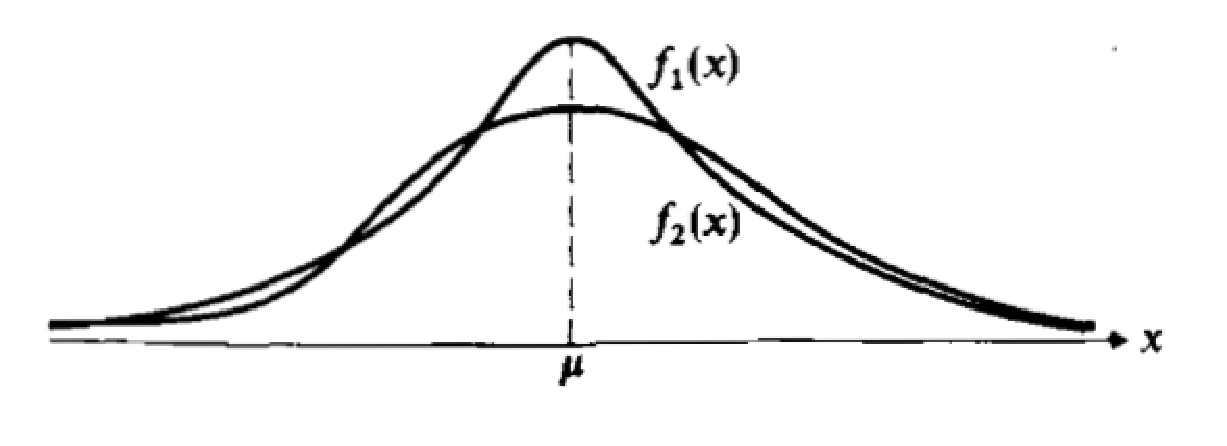
\includegraphics[scale = 0.5]{pictures/two_distributions.eps}
\caption{Pravděpodobnostní funkce $f_1(x)$ a $f_2(x)$ se shodnou střední hodnotou $\mu$}
\label{two_distributions}
\end{figure}
Lze dokázat, že rozptyl $\sigma_1^2$ pravděpodobnostní funkce $f_1(x)$ je menší než rozptyl $\sigma_2^2$ pravděpodobnostní funkce $f_2(x)$. Schéma důkazu je následující. Nechť $g(x) = f_1(x) - f_2(x)$, kde $f_1(x)$ a $f_2(x)$ splňují výše uvedenou podmínku. Protože z definice pravděpodobnostní funkce vyplývá $\int_{-\infty}^{\infty} g(x) dx = 0$, je v případě funkce $g(x)$ obsah ploch nad osou $x$ roven obsahu ploch od osou $x$. Dále je z podmínky pro funkce $f_1(x)$ a $f_2(x)$ patrné, že každý kladný element $g(x')dx'$ je vyvážen záporným elementem $g(x'')dx''$, kde $x''$ je dále od $\mu$ než $x'$. Jestliže tyto elementy násobíme $(x - \mu)^2$, jsou záporné elementy násobeny větším faktorem. Proto $\int_{-\infty}^{\infty}(x - \mu)^2 g(x) dx < 0$, pokud jsou $f_1(x)$ a $f_2(x)$ rozdílné. Z toho vyplývá $\sigma_1^2 < \sigma_2^2$.

Třetí centrální moment $\mu_3$ nazýváme mírou sešikmení. Pravděpodobnostní funkce, které jsou symetrické okolo své střední hodnoty, mají sešikmení $\mu_3 = 0$. Pravděpodobnostní funkce sešikmené do leva mají $\mu_3 < 0$. Pravděpodobnostní funkce sešikmené do prava pak mají $\mu_3 > 0$. Poněkud paradoxně nám však míra sešikmení neříká nic tvaru pravděpodobnostní funkce. Např. pravděpodobnostní funkce $f_4(x)$ na následujícím obrázku má $\mu_3 = 0$, avšak o symetrickou funkci se nejedná.
\figure[ht]\centering
\begin{pspicture}(14.0,3.0)
    \psline(0.0,0.5)(13.5,0.5)
      
    \pscurve[showpoints=false](0.0,0.6)(0.5,0.7)(1.5,2.0)(2.5,0.7)(3.0,0.6)
    \pscurve[showpoints=false](3.5,0.6)(4.0,0.7)(4.0,2.0)(6.0,0.7)(6.5,0.6)
    \pscurve[showpoints=false](7.0,0.6)(7.5,0.7)(9.0,2.0)(9.5,0.7)(10.0,0.6)
    \pscurve[showpoints=false](10.5,0.6)(11.0,0.7)(11.7,1.0)(12.0,2.0)(13.0,1.0)(13.5,0.6)

    \rput(1.5,2.3){\psframebox*{\tiny{$f_1(x): \mu = 0$}}}
    \rput(1.5,0.2){\psframebox*{\tiny{(a)}}}
    \rput(4.0,2.3){\psframebox*{\tiny{$f_2(x): \mu < 0$}}}
    \rput(5.0,0.2){\psframebox*{\tiny{(b)}}}
    \rput(9.0,2.3){\psframebox*{\tiny{$f_3(x): \mu > 0$}}}
    \rput(8.5,0.2){\psframebox*{\tiny{(c)}}}
    \rput(12.0,2.3){\psframebox*{\tiny{$f_4(x): \mu = 0$}}}
    \rput(12.0,0.2){\psframebox*{\tiny{(d)}}}

  \end{pspicture}
  \caption{Pravděpodobnostní funkce s rozdílnou mírou sešikmení}
\endfigure
Alternativním ukazatelem sešikmení je
\begin{equation*}
s = \frac{\textit{průměr - medián}}{\textit{směrodatná odchylka}}
\end{equation*}
Lze dokázat, že $-1 \le s \le 1$.

Čtvrtý centrální moment se používá jako ukazatel zakřivení, která vyjadřuje míru ``plochosti'' pravděpodobnostní funkce v okolí jejího středu. Pozitivní hodnota $\frac{\mu_4}{\sigma^4}-3$ indikuje, že daná pravděpodobnostní funkce je v okolí svého středu více ``špičatá'' než pravděpodobnostní funkce normálního rozdělení. Naopak, negativní hodnota $\frac{\mu_4}{\sigma^4}-3$ indikuje, že daná pravděpodobnostní funkce je v okolí svého středu více ``plochá'' než pravděpodobnostní funkce normálního rozdělení. Podobně jako v případě sešikmení, ani v případě zakřivení není tento ukazatel vždy směrodatný pro tvar pravděpodobnostní funkce.

Ačkoliv několik momentů může postkytnout pouze omezenou informaci o pravděpodobnostní funkci, soubor všech momentů definuje pravděpodobnostní funkci jednoznačně.

\begin{figure}[htp]
\centering
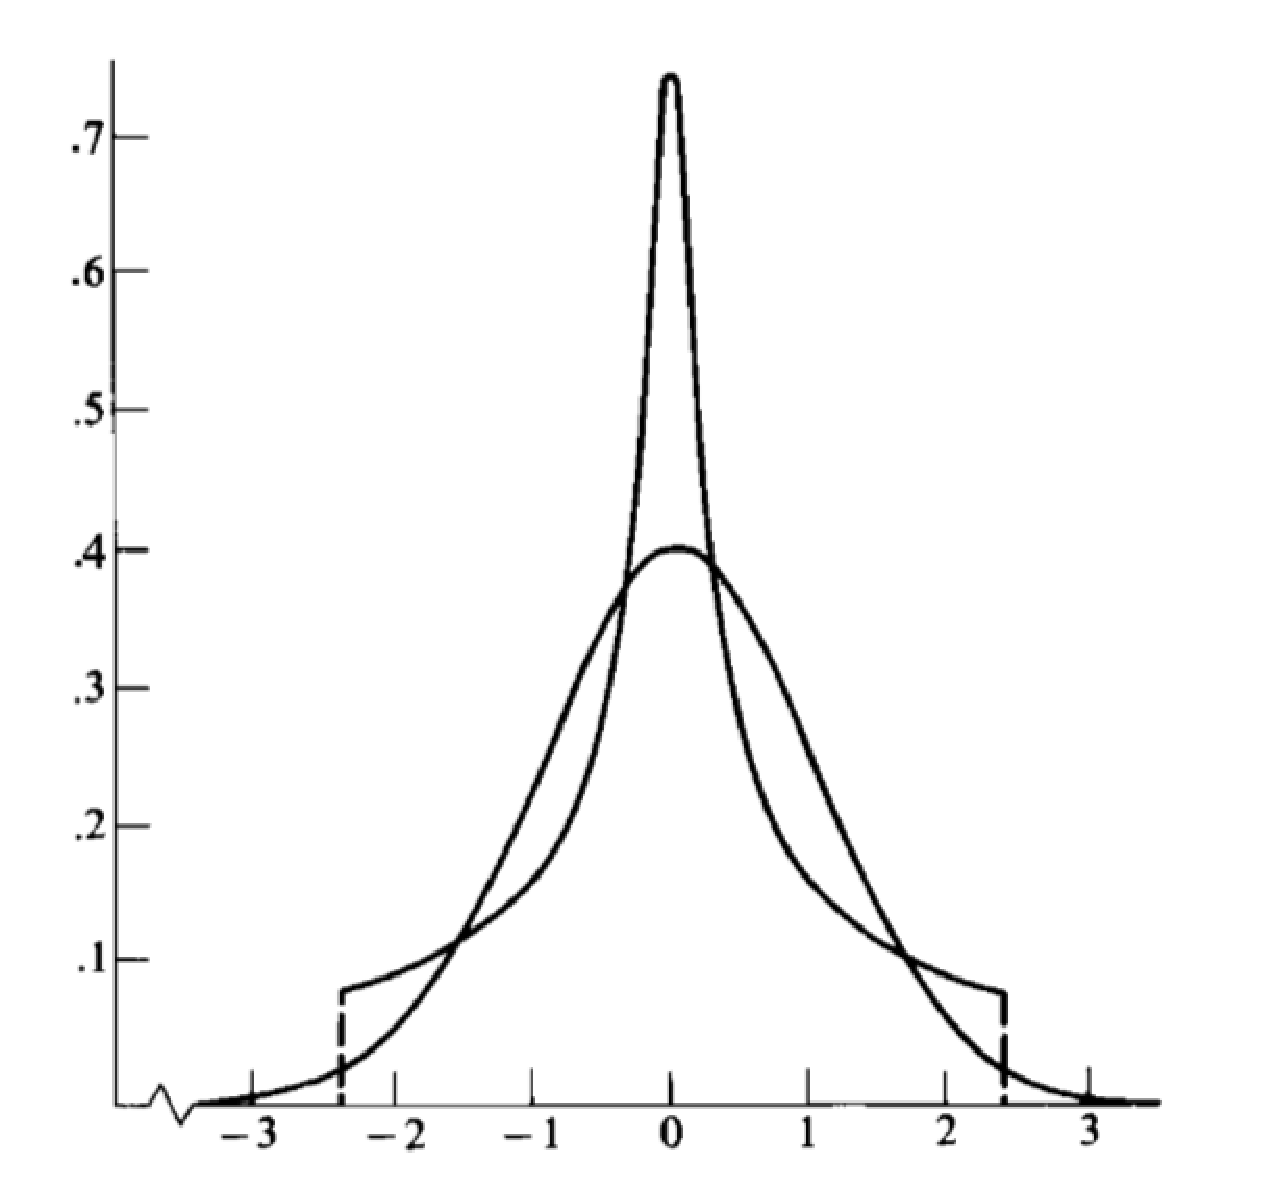
\includegraphics[scale = 0.3]{pictures/first_four_moments.eps}
\caption{Dvě pravděpodobnostní funkce se shodnými prvními čtyřmi momenty}
\label{first_four_moments}
\end{figure}

V aplikované statistice hrají klíčovou roli především první dva momenty, třetí a čtvrtý moment se používají vyjímečně a vyšší momenty pak téměr vůbec.

\begin{definition}[Faktoriální moment]
Jestliže je $X$ náhodnou veličinou, pak $r$-tý faktoriální moment $X$ je definován jako
\begin{equation*}
E[X(X-1) \cdots (X - r + 1)]
\end{equation*}
\end{definition}
Pro některé, zpravidla nespojité, náhodné veličiny je snazší vypočíst faktoriální moment než obecný popř. centrální moment. Nicméně platí, že z faktoriálního momentu lze odvodit obecný popř. centrální moment a naopak.

\begin{definition}[Momentová funkce]
Nechť je $X$ náhodná veličina s pravděpodobnostní funkcí $f_X(\cdot)$. Očekávaná hodnota $e^{tX}$ je definuje tzv. momentovou funkci, jestliže tato očekávaná hodnota existuje pro každé $t$ v intervalu $-h < t < h$ pro $h > 0$. Momentová funkce má tvar
\begin{equation*}
m(t) = E[e^{tx}] = \int_{-\infty}^{\infty} e^{tx}f_X(x)dx
\end{equation*}
je-li $X$ spojité a
\begin{equation*}
m(t) = E[e^{tx}] = \sum_x e^{tx}f_X(x)
\end{equation*}
je-li $X$ nespojité.
\end{definition}

Existuje-li momentová funkce, pak je spojitě diferenciovatelná v okolí počátku. Jestliže momentovou funkci $r$ krát derivujeme vzhledem k $t$, pak získáme
\begin{equation*}
\frac{d^r}{dt^r}m(t) = \int_{-\infty}^{\infty}x^r e^{xt}f_X(x)dx
\end{equation*}
a jestliže $r \rightarrow 0$, pak
\begin{equation*}
\frac{d^r}{dt^r}m(0) = E[X^r] = \mu_r'
\end{equation*}
Momenty pravděpodobnostní funkce tak lze získat z momentové funkce její derivací dle $t$.

Jestliže v momentové funkci nahradíme $e^{tx}$ Taylorovým rozvojem, pak získáme
\begin{equation*}
m(t) = E\big[1 + tX + \frac{1}{2!}(tX)^2 + \frac{1}{3!}(tX)^3 + \cdots \big] = 1 + \mu_1't + \frac{1}{2!}\mu_2't^2 + \cdots = \sum_{t = 0}^{\infty}\frac{1}{i!}\mu_t't^i
\end{equation*}
Z výše uvedené rovnice je patrné, že $\mu_r'$ lze získat z Taylorova rozvoje $m(t)$ jako koeficient prvku $\frac{t^r}{r!}$.

\begin{example}
Nechť je $X$ náhodná veličina s pravděpodobnostní funkcí $f_X(x) = \lambda e^{-\lambda x}I_{[0, \infty)}(x)$. Pak
\begin{equation*}
m(t) = E[e^{tX}] = \int_0^{\infty} e^{tx} \lambda e^{-\lambda x} dx = \frac{\lambda}{\lambda - t}~~~\textit{pro}~t < \lambda
\end{equation*}
a proto
\begin{equation*}
m'(t) = \frac{\lambda}{(\lambda - t)^2}~~~\textit{což implikuje}~~~m'(0) = E[X] = \frac{1}{\lambda}
\end{equation*}
\begin{equation*}
m''(t) = \frac{2 \lambda}{(\lambda - t)^3}~~~\textit{což implikuje}~~~m''(0) = E[X^2] = \frac{2}{\lambda^2}
\end{equation*}
\end{example}

\begin{example}
Uvažujme náhodnou veličinu $X$ s pravděpodobnostní funkcí $f_X(x) = x^{-2}I_{[1, \infty)}(x)$. Kdyby momentová funkce této náhodné veličiny existovala, pak by byla dána rovnicí $\int_1^{\infty}X^{-2}e^{tx}dx$. Lze však dokázat, že takovýto integrál neexistuje pro žádné $t > 0$, a proto také neexistuje tato momentová funkce.
\end{example}

\begin{definition}[Faktoriální momentová funkce]
Nechť je $X$ náhodná veličina. Faktoriální momentová funkce je definována jako $E[t^x]$, jestliže tato střední hodnota existuje.
\end{definition}

Faktoriální momentovou funkci lze použít pro generování faktoriálních momentů stejným způsobem jakým lze odvodit obecný moment z momentové funkce. Jediným rozdílem je, že $t \rightarrow 1$ namísto $t \rightarrow 0$. Tento postup někdy zjednodušuje nalezení momentu v případě nespojité pravděpodobnostní funkce.

\begin{example}
Nechť je $X$ náhodná veličina s nespojitou pravděpodobostní funkcí
\begin{equation*}
f_X(x) = \frac{e^{-\lambda}\lambda^x}{x!}
\end{equation*}
Pak
\begin{equation*}
E[t^X] = \sum_{x = 0}^{\infty} \frac{t^x e^{-\lambda} \lambda^x}{x!} = e^{-\lambda} e^{\lambda t} = e^{\lambda(t - 1)}
\end{equation*}
\begin{equation*}
\frac{d}{dt}E[t^X] = \frac{d}{dt} e^{\lambda(t-1)}=\lambda e^{\lambda (t - 1)}~~~\textit{a proto}~~~\frac{d}{dt}E[t^X] \Big|_{t = 1} = \lambda
\end{equation*}
\end{example}

Momentovou funkci lze, jak její název napovídá, použít k výpočtu momentů. Vedle toho ji však lze také použít k určení pravděpodobnostní funkce.

\begin{theorem}
Nechť jsou $X$ a $Y$ dvě náhodné veličiny s pravděpodobnostními funkcemi $f_X(\cdot)$ a $f_Y(\cdot)$. Předpokládejme, že jejich momentové funkce $m_X(t)$ a $m_Y(t)$ existují a jsou shodné pro všechna $t$ z intervalu $-h < t < h$ pro $h > 0$. Potom jsou shodné také pravděpodobnostní funkce $f_X(\cdot)$ a $f_Y(\cdot)$.
\end{theorem}
